\documentclass[12pt]{article}

\usepackage{helpers}

\begin{document}

Name: \makebox[3in]{\hrulefill
%NAME
\hrulefill}

\vfill

\begin{center}
{\huge Retest 1}

{\large April 11, 2025}
\end{center}

\testrules

\vfill

\pledge

\newpage

%BEGIN_STANDARD_DR

\section*{Data Representation}

Demonstrate understanding of numeric and non-numeric data through conversions and operations on such data. Please show your work!

\begin{enumerate}
\item Convert the (unsigned) binary integer 0b00101101 to decimal.
\vfill

\item Convert the two's complement binary integer 0b11110100 to decimal.
\vfill

\item Convert the decimal integer -45 to two's complement binary.
\vfill

\pagebreak

\item Convert the hexadecimal number 0x28 to binary.
\vfill

\item Compute the following subtraction of two's complement binary integers: 0b11101000 - 0b10011111. 
\vfill

\item Write the string ``CS 241'' as a sequence of ASCII values. An ASCII table is included at the end of this test.
\vfill
\end{enumerate}

\vfill

\standardsfooter

\newpage

%END_STANDARD_DR

%BEGIN_STANDARD_LR

\section*{Logic Representation}

Demonstrate understanding of boolean expressions and operations, logic circuits through computation and modeling.

\begin{enumerate}
\item Consider the boolean function $f(A,B) = (A\textrm{ and }B)\textrm{ OR }(A\textrm{ xor }B)$. Make a truth table for this function.
\vfill

\item The function $f$ above is equivalent to a basic boolean function. Which boolean function is it equivalent to?
\vfill

\pagebreak

\item Draw a logic circuit with two 1-bit inputs, $A$ and $B$, and one output, $C$. The output $C$ is 1 if $A$ and $B$ are equal. Otherwise, $C$ is 0.
\vfill

\item Draw a logic circuit with three 1-bit inputs, $A$, $B$, and $C$, representing the bits of a 2-bit binary integer $AB$ and a 1-bit binary integer $C$. There should be three 1-bit outputs, $D$, $E$, and $F$, representing the bits of the result $DEF = AB + C$.
\vfill
\end{enumerate}

\vfill

\standardsfooter

\newpage

%END_STANDARD_LR

%BEGIN_STANDARD_AP

\section*{Assembly Programming}

Demonstrate understanding of assembly programming by writing a program using global variables, local variables, input with \texttt{scanf}, and/or output with \texttt{printf}.

Write an assembly program called \texttt{adder.s} that does the following:
\begin{itemize}
\item Ask the user to enter a number, and store their response in a \textbf{global variable} called \texttt{num1}.
\item Ask the user to enter a number again, and store their response in another \textbf{global variable} called \texttt{num2}.
\item Compute the sum of \texttt{num1} and \texttt{num2}, and storing the result to a \textbf{global variable} called \texttt{total}.
\item Print the sentence ``The sum of \{num1\} and \{num2\} is \{total\}'', where \{num1\} is replaced with the value of \texttt{num1}, \{num2\} is replaced with the value of \texttt{num2}, and \{total\} is replaced with the value of \texttt{total}. For example, if the user entered 2 and 3, the program would print ``The sum of 2 and 3 is 5''.
\end{itemize}
Below are comments outlining the structure of this program. You may write your assembly code between the comments, or on a separate sheet of paper. If you write on a separate sheet of paper, you do not need to rewrite the comments.

\textbf{square.s}

\begin{verbatim}
@ Global constants
@ prompt: string asking the user to enter a number


@ input_string: formatting string for reading the user's input


@ print_report: formatting string for reporting the sum of the user's numbers


@ Global variables


@ main

     @ set up stack frame for main

     
     @ ask the user to enter a number

     
     @ store the response in num1

     
     @ ask the user to enter a number again

     
     @ store the response in num2


     @ load the values of num1 and num2, add them, and store the result in total

     
     @ print a sentence saying what the sum of the numbers is

     
     @ return 0

     @ tear down stack frame for main


@ Pointers
@ pointers to strings

\end{verbatim}

\vfill

\standardsfooter

\newpage

%END_STANDARD_AP

%BEGIN_STANDARD_HC

\section*{Hardware Components}

Demonstrate understanding of hardware components and their purposes through answering conceptual questions and identifying components.

\begin{enumerate}
\item What are the two main subcomponents of the CPU? What does each of them do?
\vfill
\item What is the role of a register in a computer?
\vfill
\item What is the role of main memory in a computer?
\vfill
\item What is a byte?
\vfill
\item What is a processor's clock cycle time? What is the relationship between clock cycle time and clock rate?
\vfill

\pagebreak

For each of the following, include which hardware components are involved, information sent on the address, control, and/or data bus, and the use of and updates to special registers.
\item Write a detailed description of what happens in the fetch phase of instruction execution in the von Neumann architecture.
\vfill
\item Write a detailed description of what happens in the decode phase of instruction execution in the von Neumann architecture.
\vfill
\item Write a detailed description of what happens in the execute phase of instruction execution in the von Neumann architecture.
\vfill
\item Write a detailed description of what happens in the store phase of instruction execution in the von Neumann architecture.
\vfill
\end{enumerate}

\vfill

\standardsfooter

%END_STANDARD_HC

\newpage

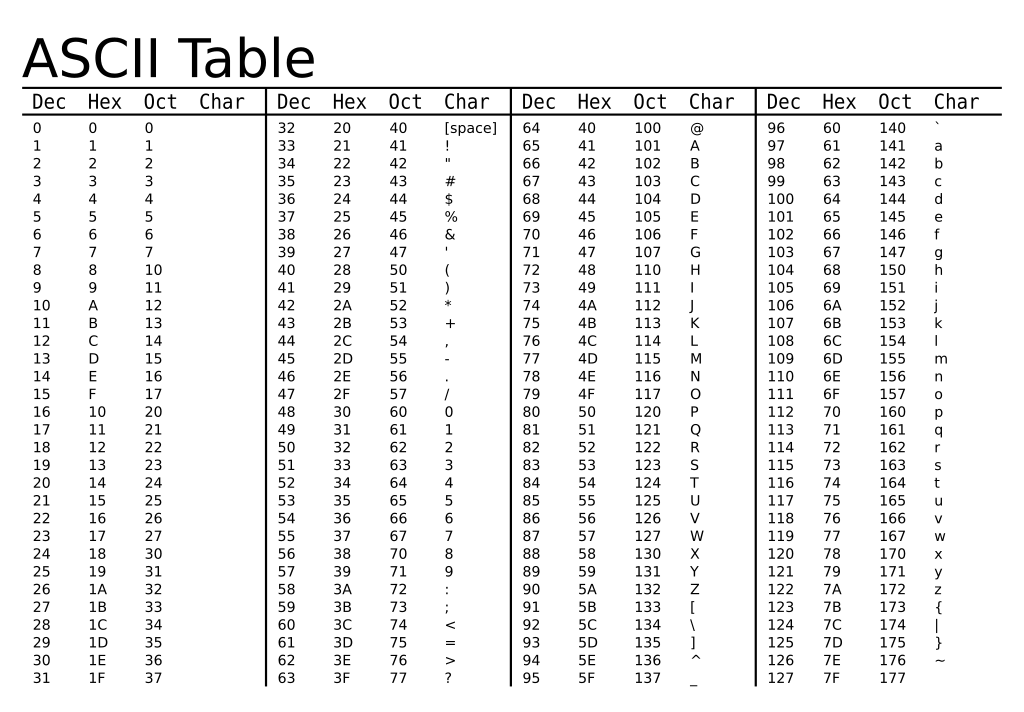
\includegraphics[height=\textheight]{ascii-table.png}

\end{document}